\chapter{Curvas de operaciones desagregadas por secuencia}\label{chap:Apendice_2}

Se incluyen el resultado obtenido por secuencias de cada algoritmo para $\alpha=0.001$ y $\alpha=0.0002$.

%\section{Curva operaciones para $\alpha=0.001$}

%\begin{figure}[!ht]
%\centering
%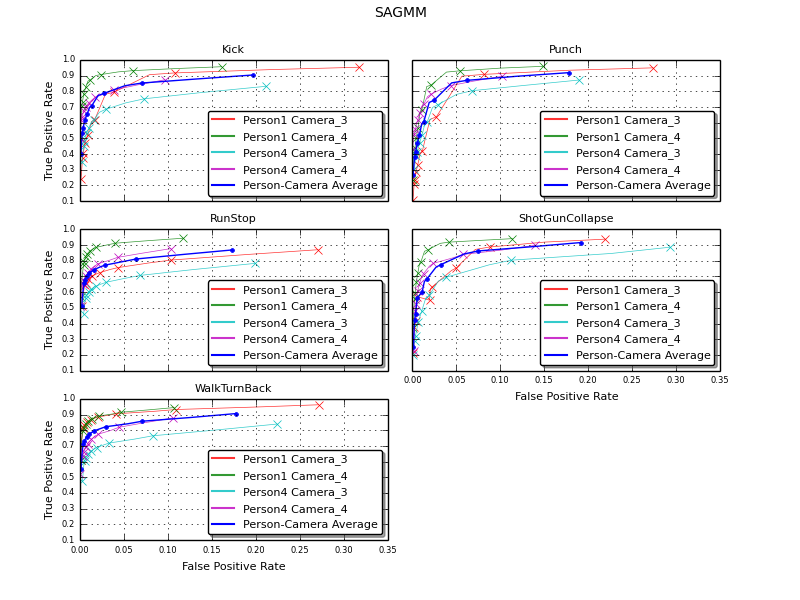
\includegraphics{img/SAGMM_Actions_3-2}
%\caption{Pesos pixeles falso positivo y negativo}
%\label{fig:Contexto espacial pesos para pixeles falso positivo y negativo}
%\end{figure}


\begin{figure}[!ht]
\centering     %%% not \center
\subfigure[Kick]%
{\label{fig:SAGMM_Kick}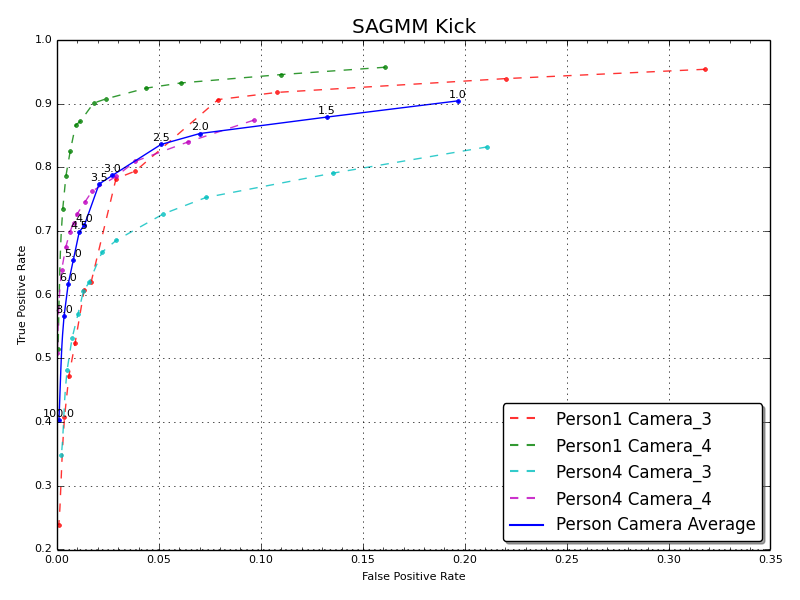
\includegraphics[width=80mm]{img/ap2/SAGMM/KICK_P-C_1-1}}
\subfigure[Punch]
{\label{fig:SAGMM_Punch}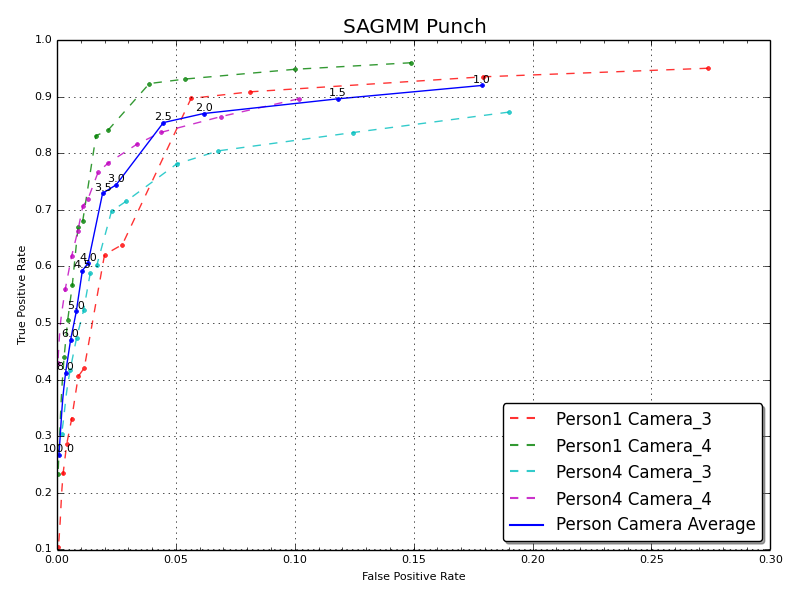
\includegraphics[width=80mm]{img/ap2/SAGMM/PUNCH_P-C_1-1}}
\subfigure[RunStop]
{\label{fig:SAGMM_RunStop}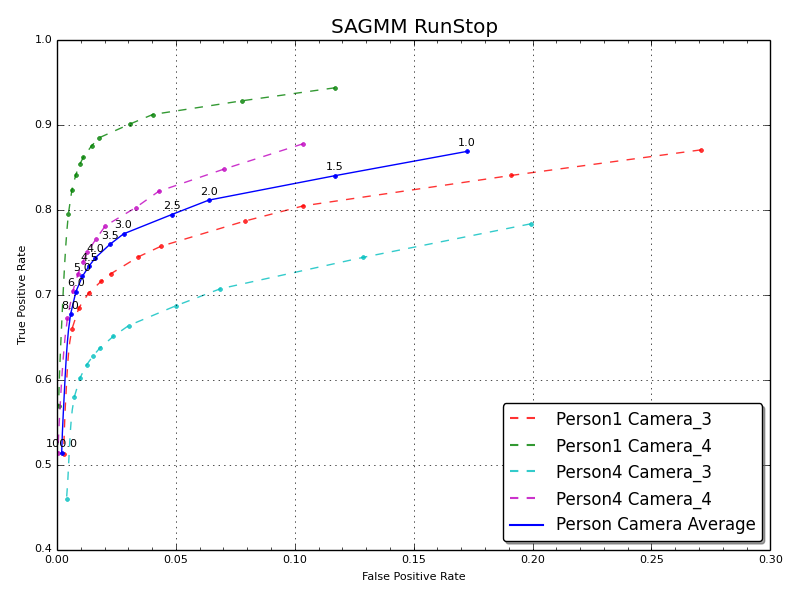
\includegraphics[width=80mm]{img/ap2/SAGMM/RUNSTOP_P-C_1-1}}
\subfigure[ShotGunCollapse]
{\label{fig:SAGMM_ShotGunCollapse}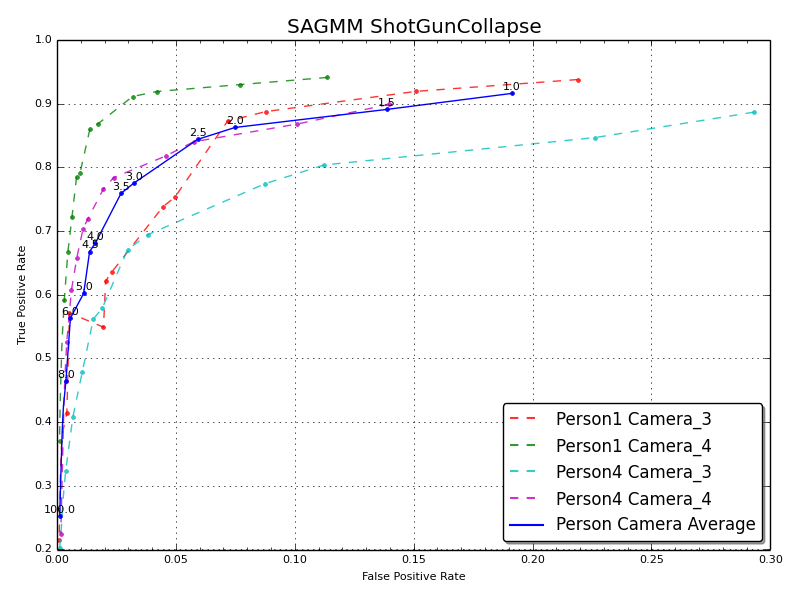
\includegraphics[width=80mm]{img/ap2/SAGMM/SHOTGUNCOLLAPSE_P-C_1-1}}
\subfigure[WalkTurnBack]
{\label{fig:SAGMM_WalkTurnBack}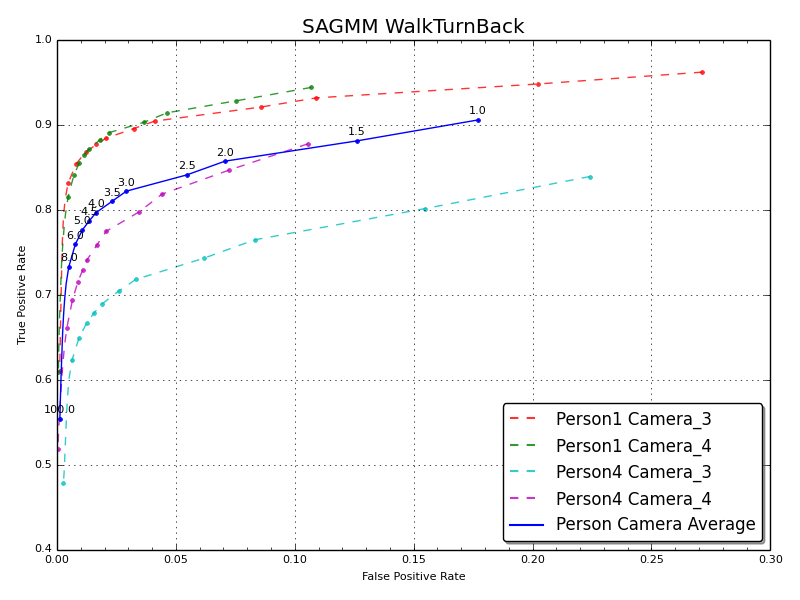
\includegraphics[width=80mm]{img/ap2/SAGMM/WALKTURNBACK_P-C_1-1}}
\caption[Gráfica resultado global algoritmo SAGMM consolidado por acción]{Resultado global separado por acción de algoritmo SAGMM}
\label{fig:SAGMM_actions}
\end{figure}


\begin{figure}[!ht]
\centering     %%% not \center
\subfigure[Person1 Camera3]%
{\label{fig:SAGMM_P1C3}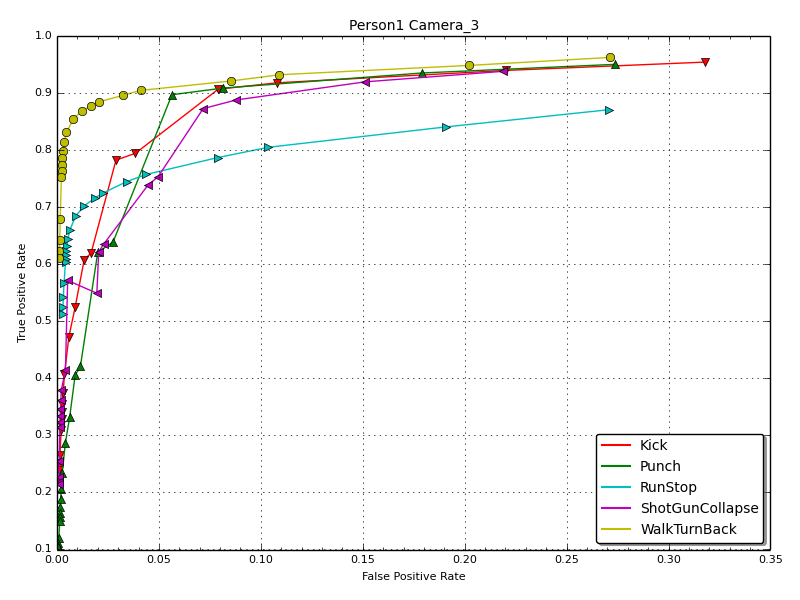
\includegraphics[width=80mm]{img/ap2/SAGMM/P1C3}}
\subfigure[Person1 Camera4]
{\label{fig:SAGMM_P1C4}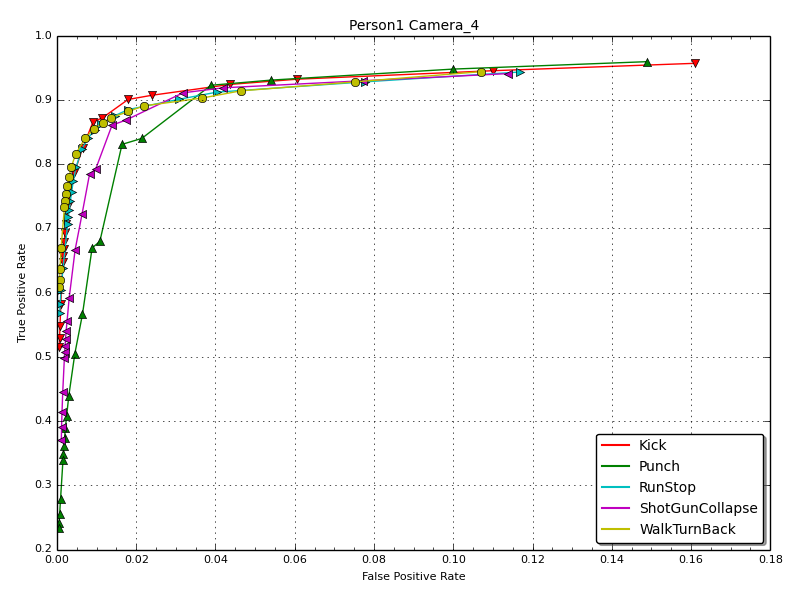
\includegraphics[width=80mm]{img/ap2/SAGMM/P1C4}}
\subfigure[Person4 Camera3]
{\label{fig:SAGMM_P4C3}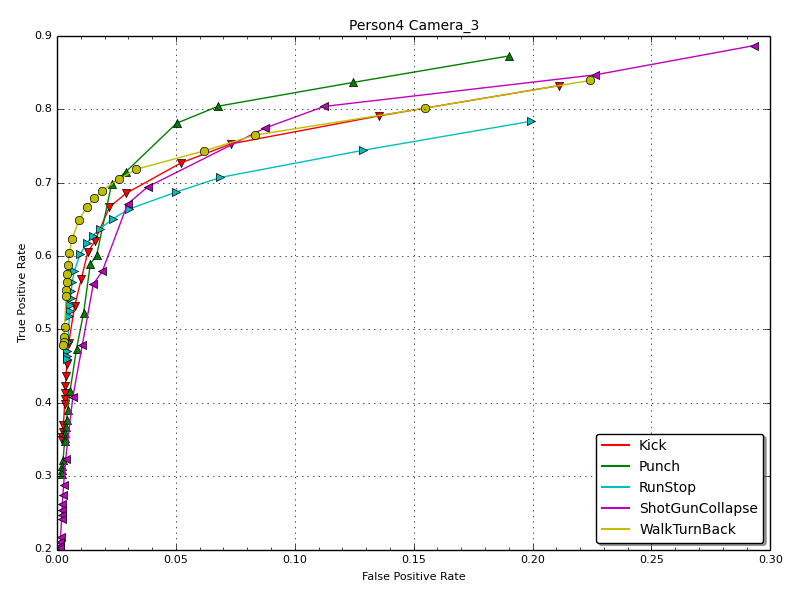
\includegraphics[width=80mm]{img/ap2/SAGMM/P4C3}}
\subfigure[Person4 Camera4]
{\label{fig:SAGMM_P4C4}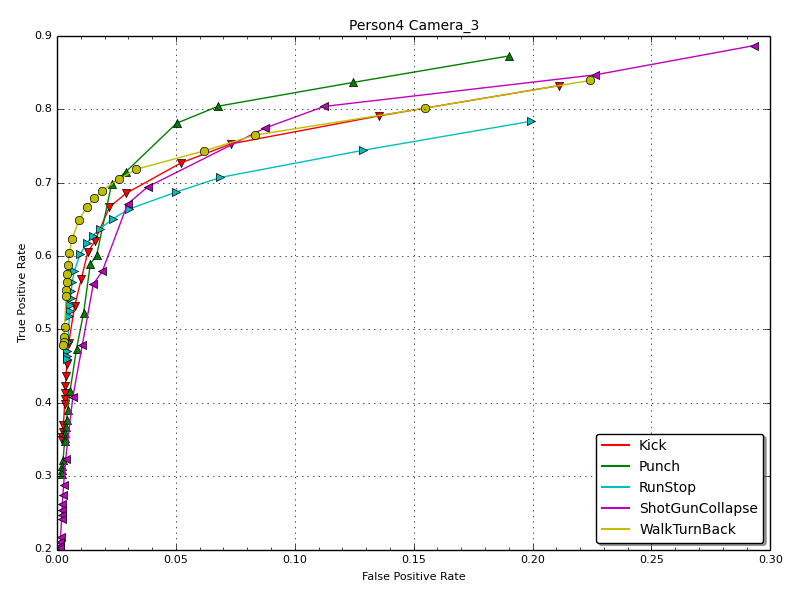
\includegraphics[width=80mm]{img/ap2/SAGMM/P4C3}}
\caption[Resultados globales de la ejecución del algoritmo SAGMM separado por actor y camara.]{Resultados globales de la ejecución del algoritmo SAGMM separado por actor y camara. \textit{Person1} muestra un buen desempeño  }
\label{fig:SAGMM_PC}
\end{figure}


\begin{figure}[!ht]
\centering     %%% not \center
\subfigure[Kick]%
{\label{fig:NP_Kick}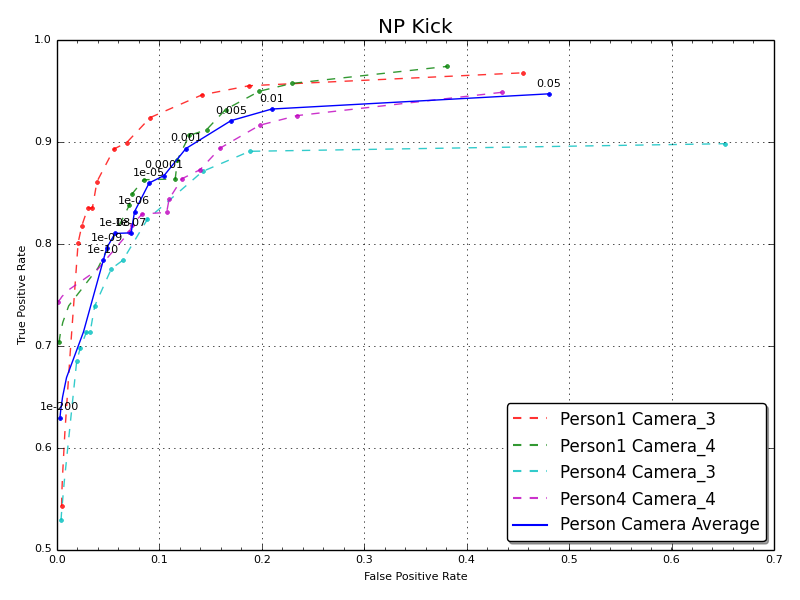
\includegraphics[width=80mm]{img/ap2/NP/KICK_P-C_1-1}}
\subfigure[Punch]
{\label{fig:NP_Punch}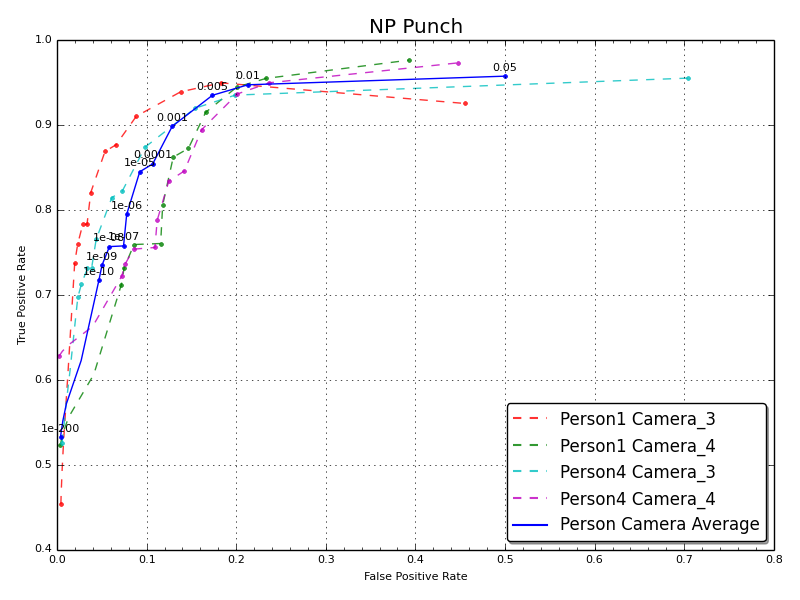
\includegraphics[width=80mm]{img/ap2/NP/PUNCH_P-C_1-1}}
\subfigure[RunStop]
{\label{fig:NP_RunStop}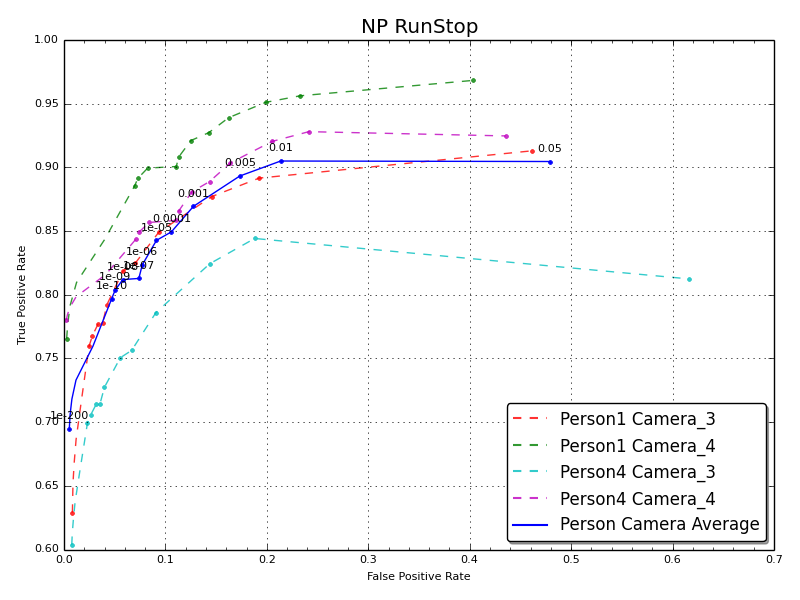
\includegraphics[width=80mm]{img/ap2/NP/RUNSTOP_P-C_1-1}}
\subfigure[ShotGunCollapse]
{\label{fig:NP_ShotGunCollapse}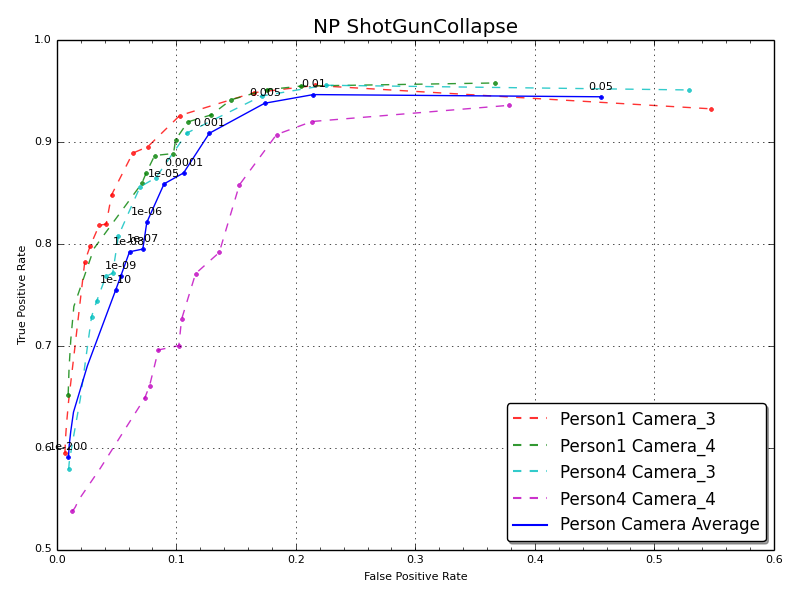
\includegraphics[width=80mm]{img/ap2/NP/SHOTGUNCOLLAPSE_P-C_1-1}}
\subfigure[WalkTurnBack]
{\label{fig:NP_WalkTurnBack}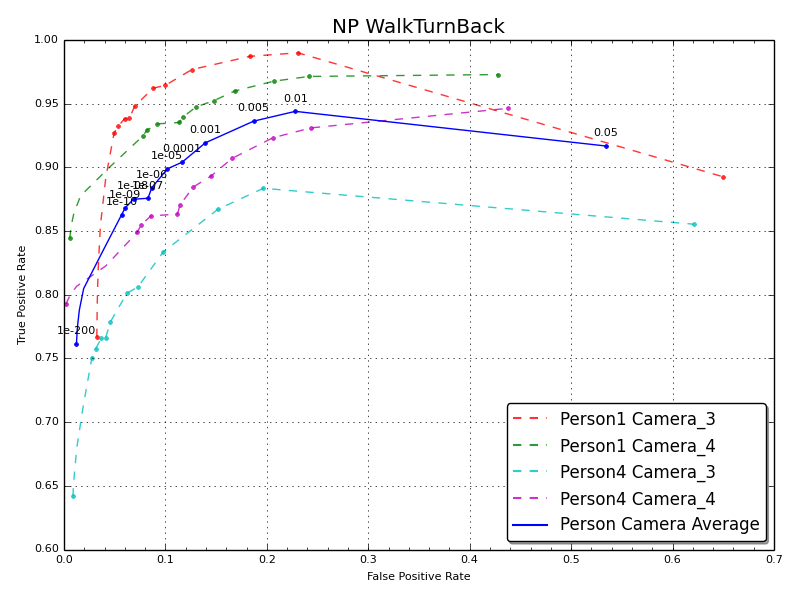
\includegraphics[width=80mm]{img/ap2/NP/WALKTURNBACK_P-C_1-1}}
\caption[Gráfica resultado global algoritmo NP consolidado por acción]{Resultado global separado por acción de algoritmo NP}
\label{fig:NP_actions}
\end{figure}


\begin{figure}[!ht]
\centering     %%% not \center
\subfigure[Person1 Camera3]%
{\label{fig:NP_P1C3}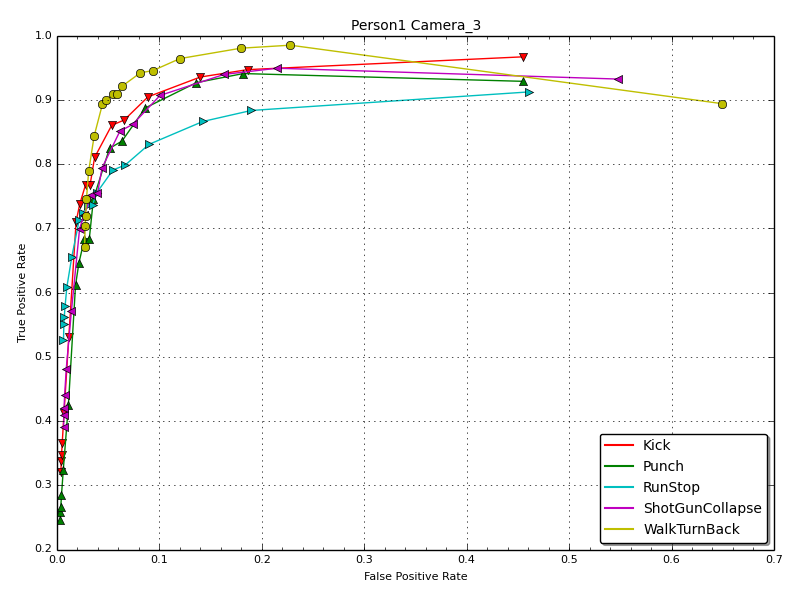
\includegraphics[width=80mm]{img/ap2/NP/P1C3}}
\subfigure[Person1 Camera4]
{\label{fig:NP_P1C4}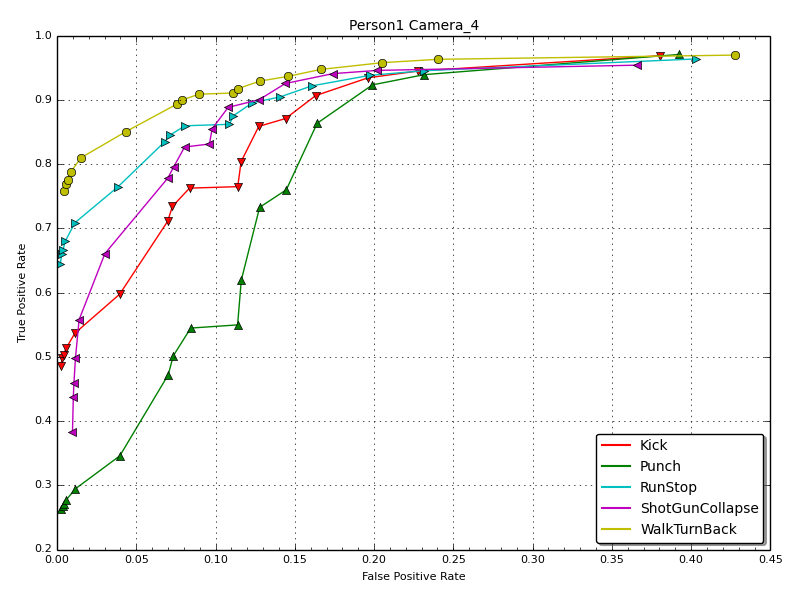
\includegraphics[width=80mm]{img/ap2/NP/P1C4}}
\subfigure[Person4 Camera3]
{\label{fig:NP_P4C3}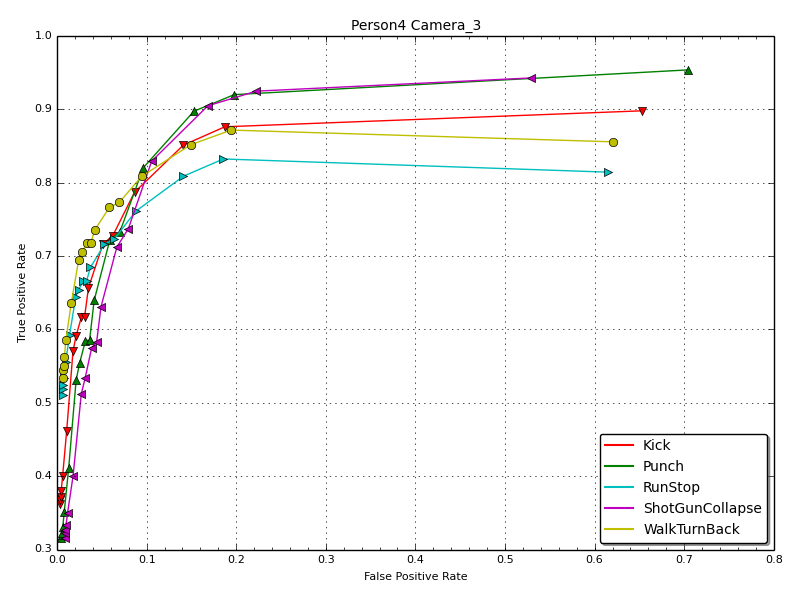
\includegraphics[width=80mm]{img/ap2/NP/P4C3}}
\subfigure[Person4 Camera4]
{\label{fig:NP_P4C4}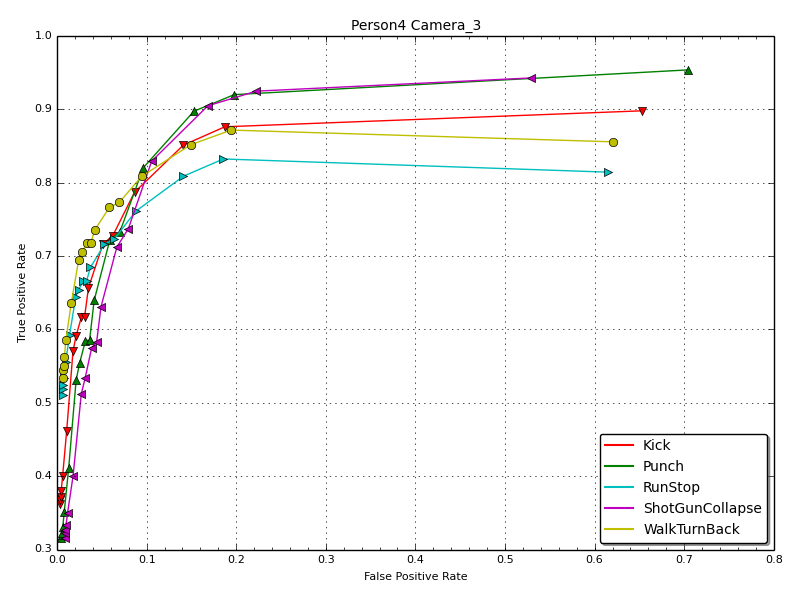
\includegraphics[width=80mm]{img/ap2/NP/P4C3}}
\caption[Resultados globales de la ejecución del algoritmo NP separado por actor y camara.]{Resultados globales de la ejecución del algoritmo NP separado por actor y camara. \textit{Person1} muestra un buen desempeño  }
\label{fig:NP_PC}
\end{figure}



\begin{figure}[!ht]
\centering     %%% not \center
\subfigure[Kick]%
{\label{fig:UCV_STAIRCASE_Kick}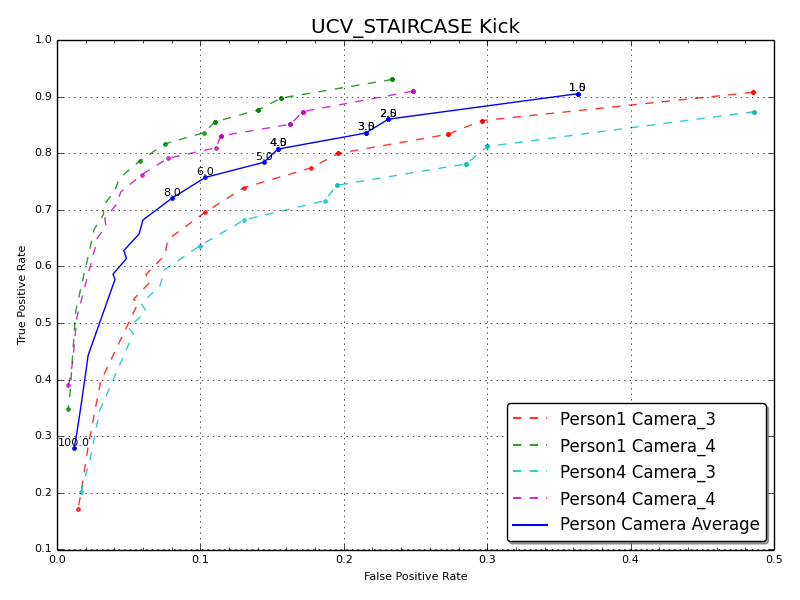
\includegraphics[width=80mm]{img/ap2/UCV_STAIRCASE/KICK_P-C_1-1}}
\subfigure[Punch]
{\label{fig:UCV_STAIRCASE_Punch}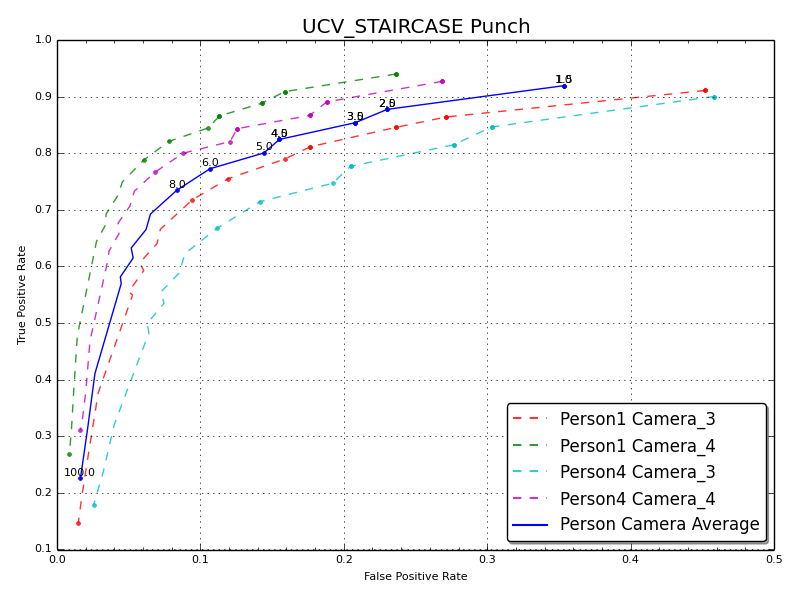
\includegraphics[width=80mm]{img/ap2/UCV_STAIRCASE/PUNCH_P-C_1-1}}
\subfigure[RunStop]
{\label{fig:UCV_STAIRCASE_RunStop}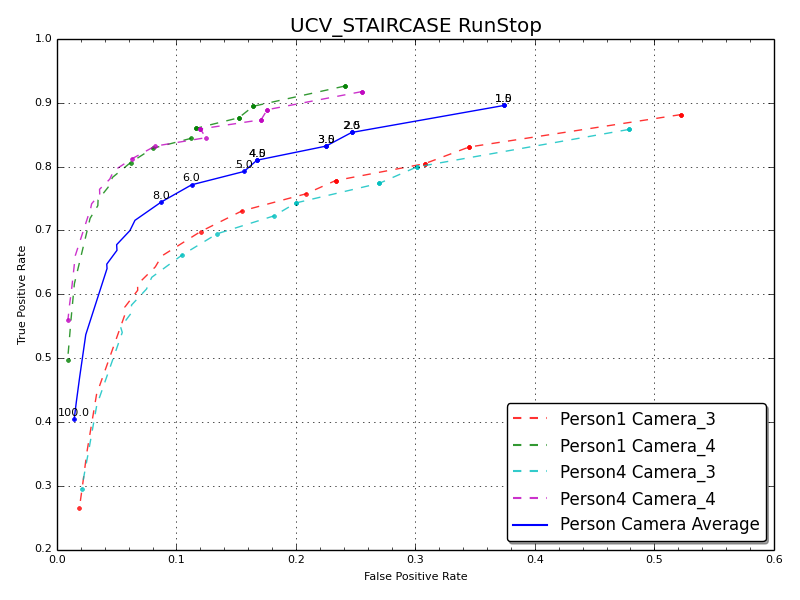
\includegraphics[width=80mm]{img/ap2/UCV_STAIRCASE/RUNSTOP_P-C_1-1}}
\subfigure[ShotGunCollapse]
{\label{fig:UCV_STAIRCASE_ShotGunCollapse}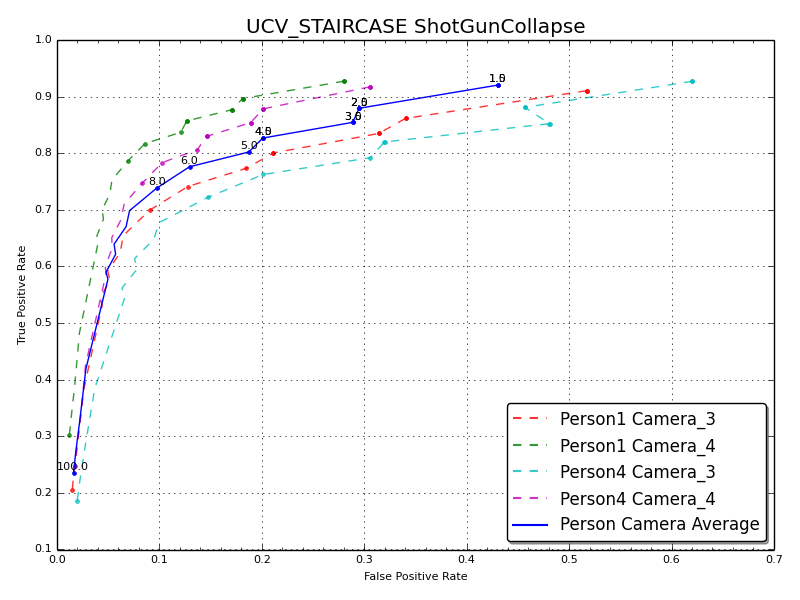
\includegraphics[width=80mm]{img/ap2/UCV_STAIRCASE/SHOTGUNCOLLAPSE_P-C_1-1}}
\subfigure[WalkTurnBack]
{\label{fig:UCV_STAIRCASE_WalkTurnBack}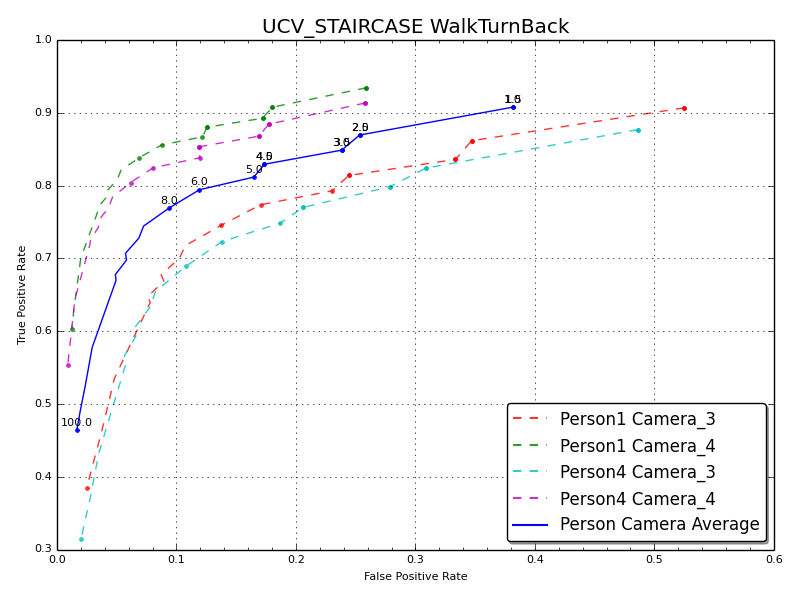
\includegraphics[width=80mm]{img/ap2/UCV_STAIRCASE/WALKTURNBACK_P-C_1-1}}
\caption[Gráfica resultado global algoritmo UCV\_STAIRCASE consolidado por acción]{Resultado global separado por acción de algoritmo UCV\_STAIRCASE}
\label{fig:UCV_STAIRCASE_actions}
\end{figure}


\begin{figure}[!ht]
\centering     %%% not \center
\subfigure[Person1 Camera3]%
{\label{fig:UCV_STAIRCASE_P1C3}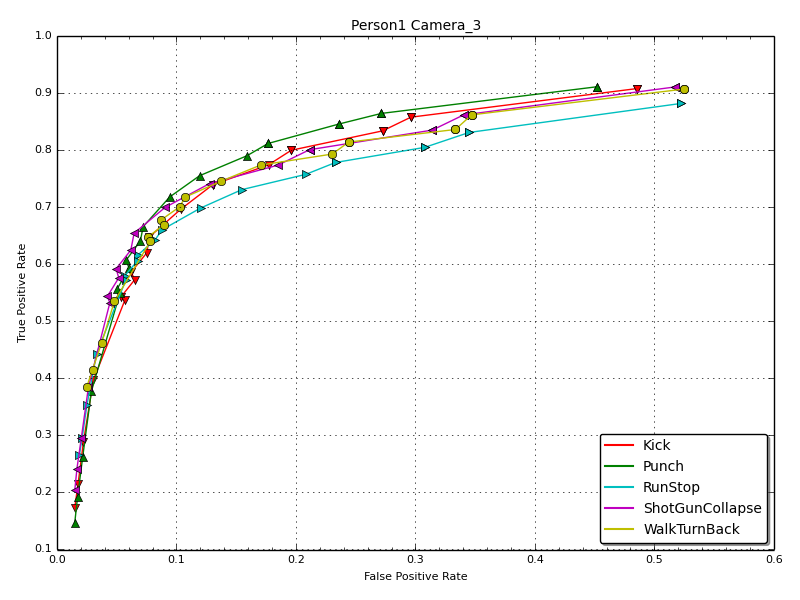
\includegraphics[width=80mm]{img/ap2/UCV_STAIRCASE/P1C3}}
\subfigure[Person1 Camera4]
{\label{fig:UCV_STAIRCASE_P1C4}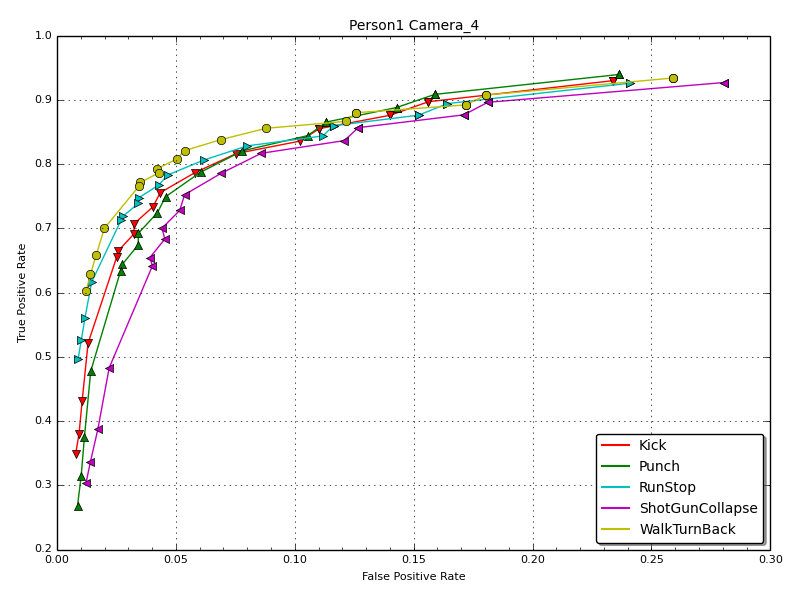
\includegraphics[width=80mm]{img/ap2/UCV_STAIRCASE/P1C4}}
\subfigure[Person4 Camera3]
{\label{fig:UCV_STAIRCASE_P4C3}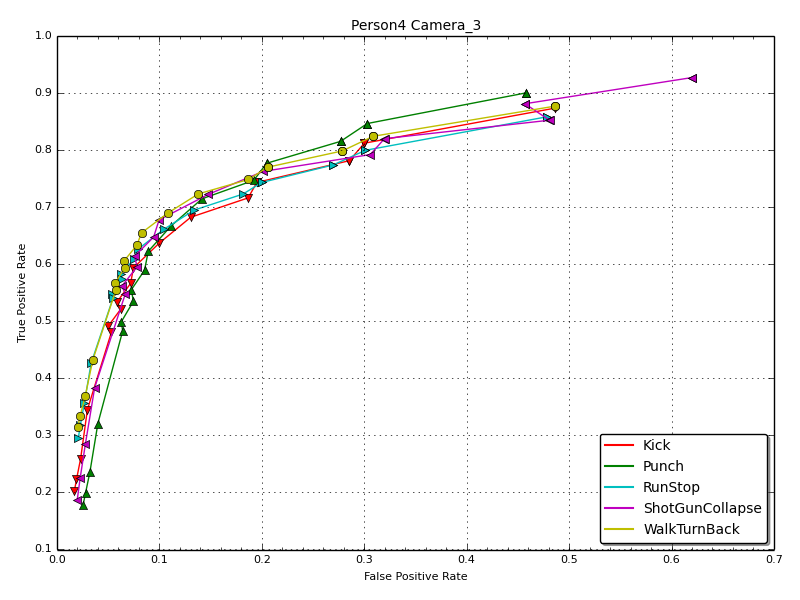
\includegraphics[width=80mm]{img/ap2/UCV_STAIRCASE/P4C3}}
\subfigure[Person4 Camera4]
{\label{fig:UCV_STAIRCASE_P4C4}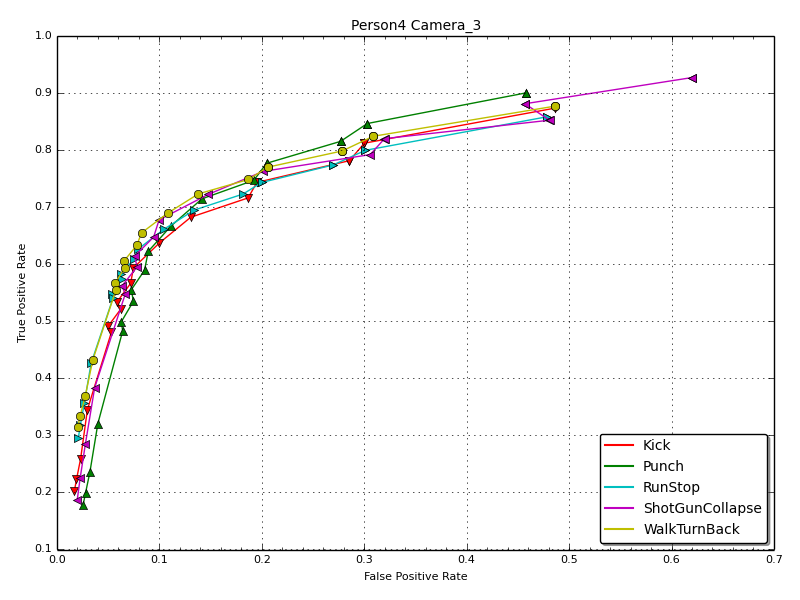
\includegraphics[width=80mm]{img/ap2/UCV_STAIRCASE/P4C3}}
\caption[Resultados globales de la ejecución del algoritmo UCV\_STAIRCASE separado por actor y camara.]{Resultados globales de la ejecución del algoritmo UCV\_STAIRCASE separado por actor y camara. \textit{Person1} muestra un buen desempeño  }
\label{fig:UCV_STAIRCASE_PC}
\end{figure}

\begin{figure}[!ht]
\centering     %%% not \center
\subfigure[Kick]%
{\label{fig:UCV_LINEAR_Kick}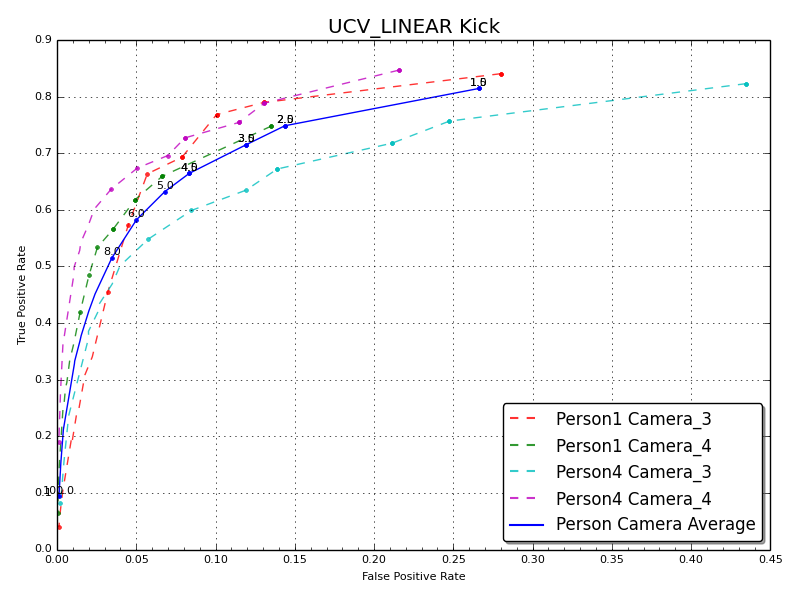
\includegraphics[width=80mm]{img/ap2/UCV_LINEAR/KICK_P-C_1-1}}
\subfigure[Punch]
{\label{fig:UCV_LINEAR_Punch}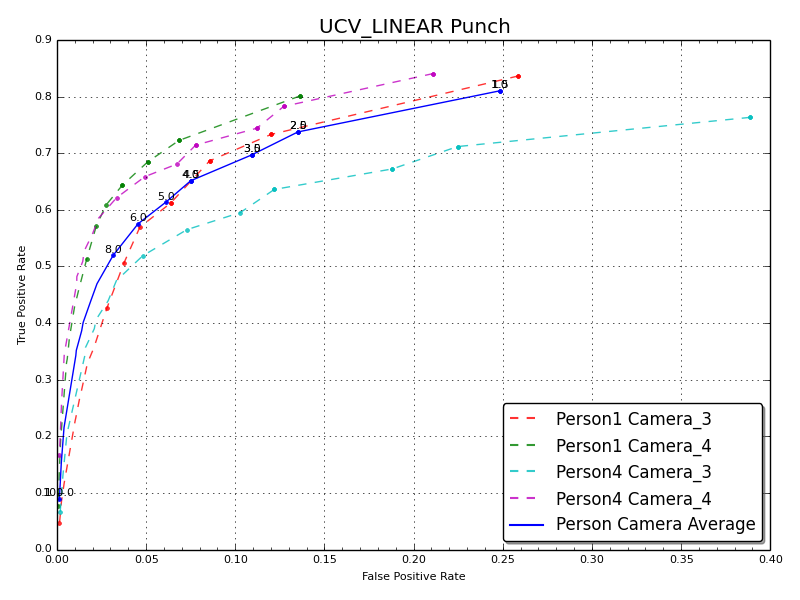
\includegraphics[width=80mm]{img/ap2/UCV_LINEAR/PUNCH_P-C_1-1}}
\subfigure[RunStop]
{\label{fig:UCV_LINEAR_RunStop}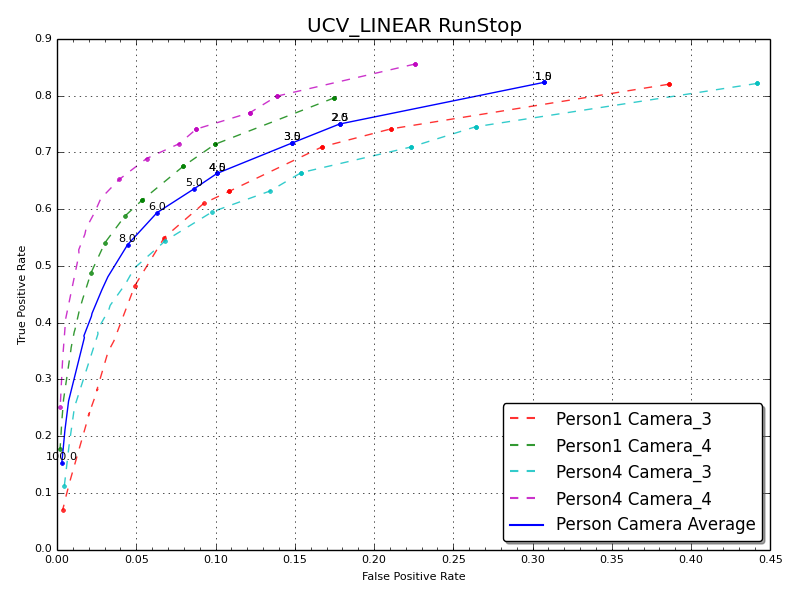
\includegraphics[width=80mm]{img/ap2/UCV_LINEAR/RUNSTOP_P-C_1-1}}
\subfigure[ShotGunCollapse]
{\label{fig:UCV_LINEAR_ShotGunCollapse}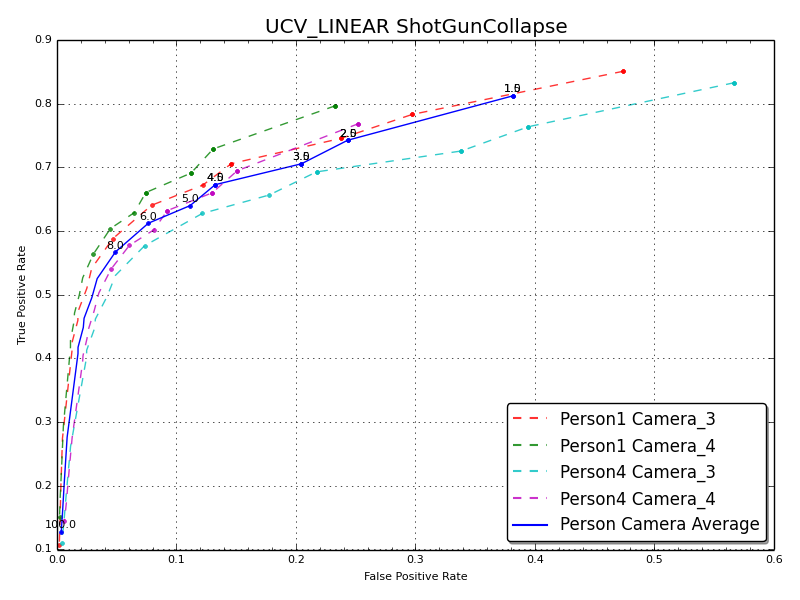
\includegraphics[width=80mm]{img/ap2/UCV_LINEAR/SHOTGUNCOLLAPSE_P-C_1-1}}
\subfigure[WalkTurnBack]
{\label{fig:UCV_LINEAR_WalkTurnBack}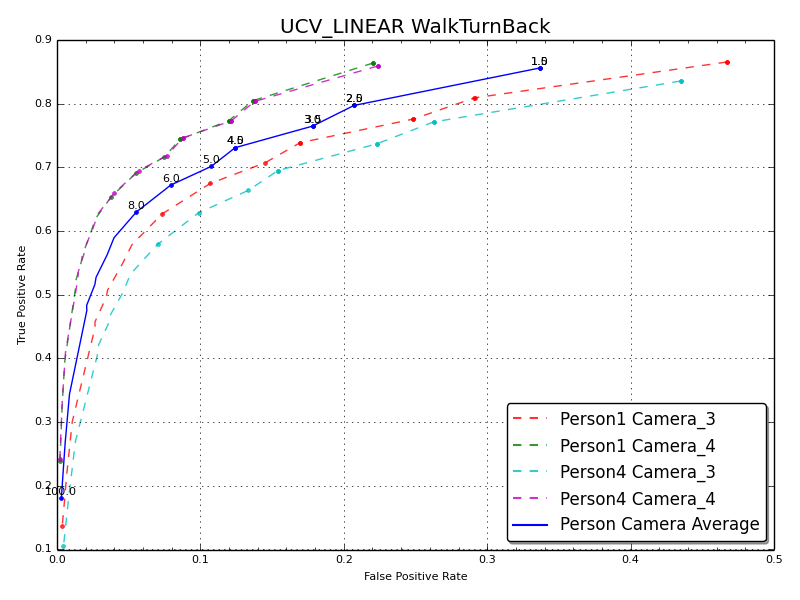
\includegraphics[width=80mm]{img/ap2/UCV_LINEAR/WALKTURNBACK_P-C_1-1}}
\caption[Gráfica resultado global algoritmo UCV\_LINEAR consolidado por acción]{Resultado global separado por acción de algoritmo UCV\_LINEAR}
\label{fig:UCV_LINEAR_actions}
\end{figure}


\begin{figure}[!ht]
\centering     %%% not \center
\subfigure[Person1 Camera3]%
{\label{fig:UCV_LINEAR_P1C3}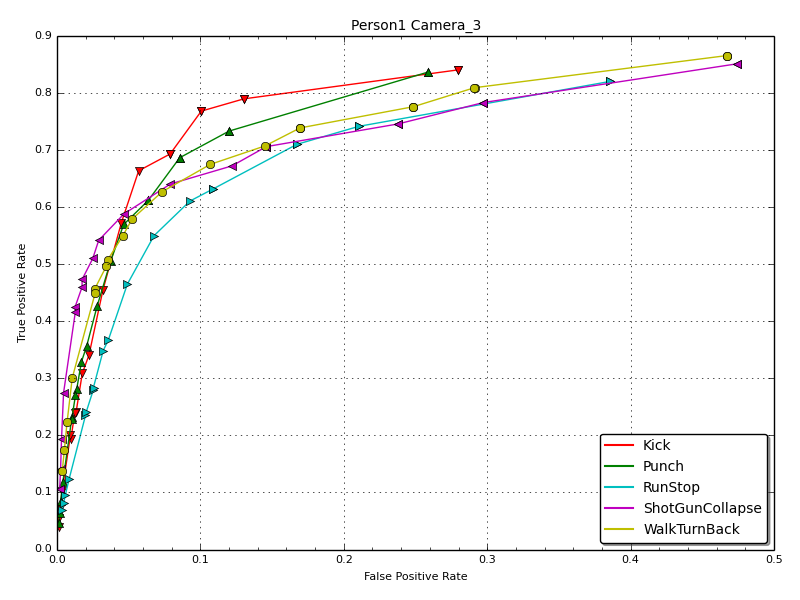
\includegraphics[width=80mm]{img/ap2/UCV_LINEAR/P1C3}}
\subfigure[Person1 Camera4]
{\label{fig:UCV_LINEAR_P1C4}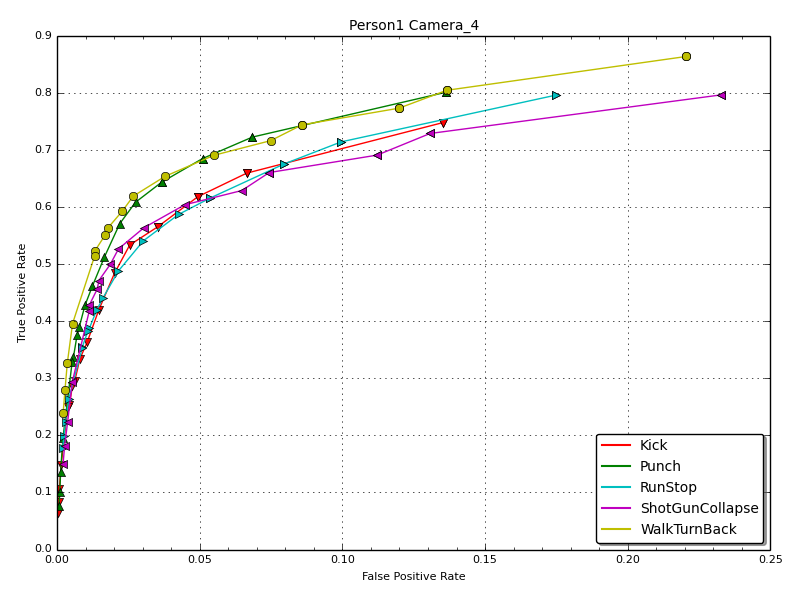
\includegraphics[width=80mm]{img/ap2/UCV_LINEAR/P1C4}}
\subfigure[Person4 Camera3]
{\label{fig:UCV_LINEAR_P4C3}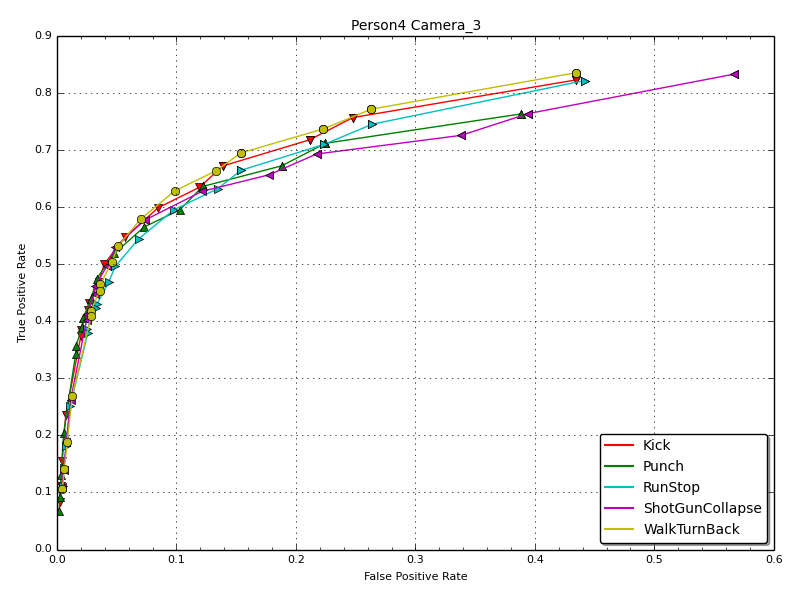
\includegraphics[width=80mm]{img/ap2/UCV_LINEAR/P4C3}}
\subfigure[Person4 Camera4]
{\label{fig:UCV_LINEAR_P4C4}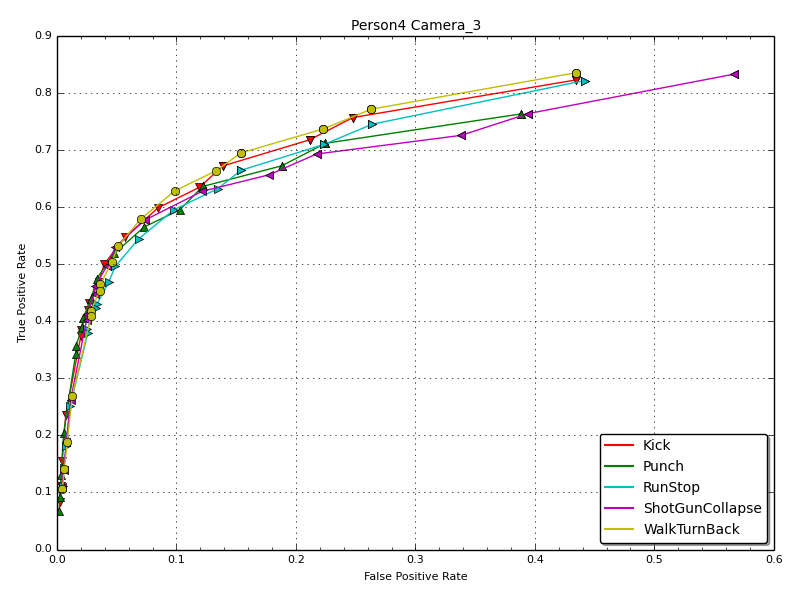
\includegraphics[width=80mm]{img/ap2/UCV_LINEAR/P4C3}}
\caption[Resultados globales de la ejecución del algoritmo UCV\_LINEAR separado por actor y camara.]{Resultados globales de la ejecución del algoritmo UCV\_LINEAR separado por actor y camara. \textit{Person1} muestra un buen desempeño  }
\label{fig:UCV_LINEAR_PC}
\end{figure}






\begin{figure}[!ht]
\centering     %%% not \center
\subfigure[Kick]%
{\label{fig:MOG2_Kick}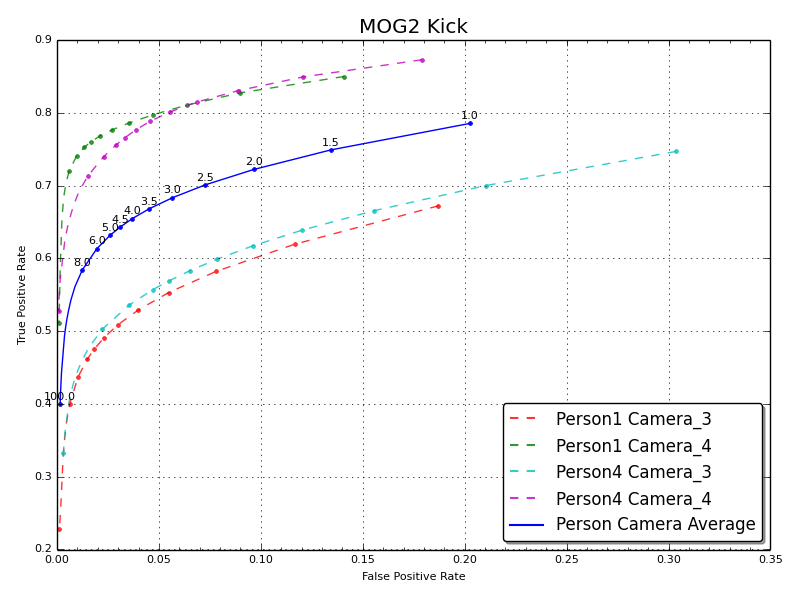
\includegraphics[width=80mm]{img/ap2/MOG2/KICK_P-C_1-1}}
\subfigure[Punch]
{\label{fig:MOG2_Punch}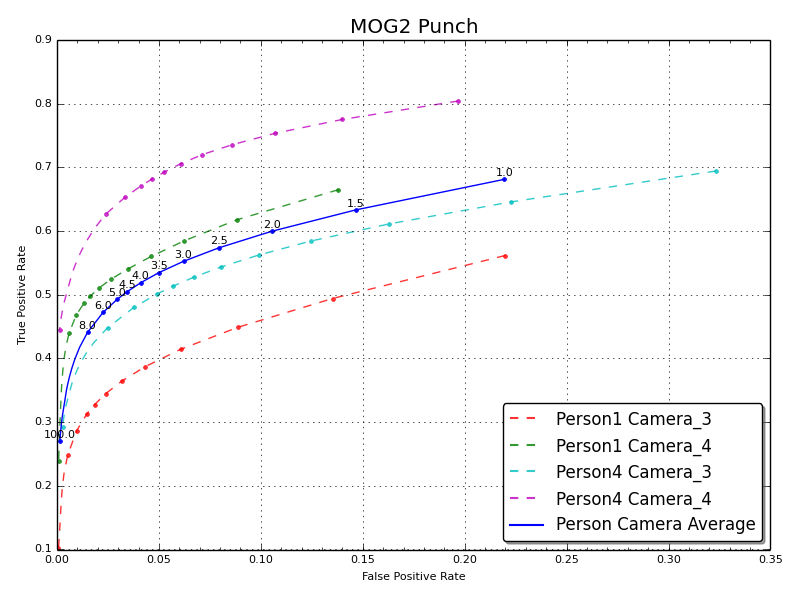
\includegraphics[width=80mm]{img/ap2/MOG2/PUNCH_P-C_1-1}}
\subfigure[RunStop]
{\label{fig:MOG2_RunStop}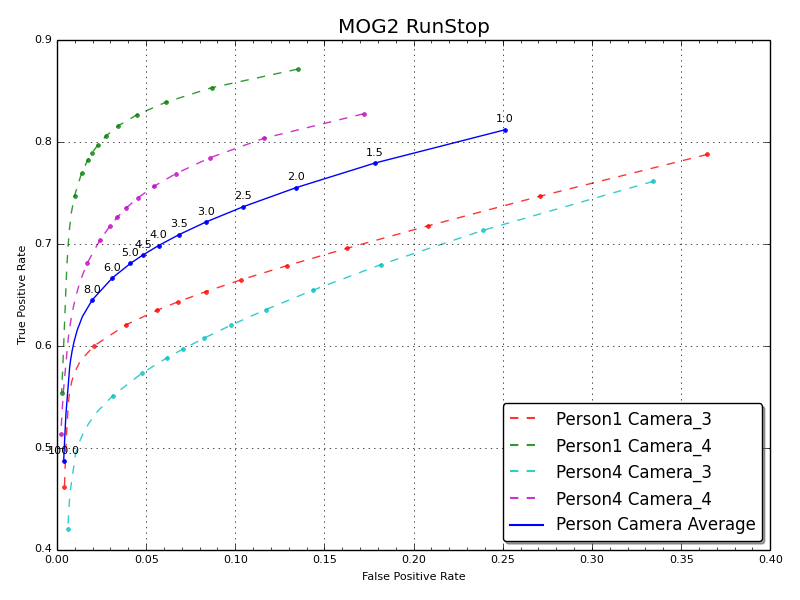
\includegraphics[width=80mm]{img/ap2/MOG2/RUNSTOP_P-C_1-1}}
\subfigure[ShotGunCollapse]
{\label{fig:MOG2_ShotGunCollapse}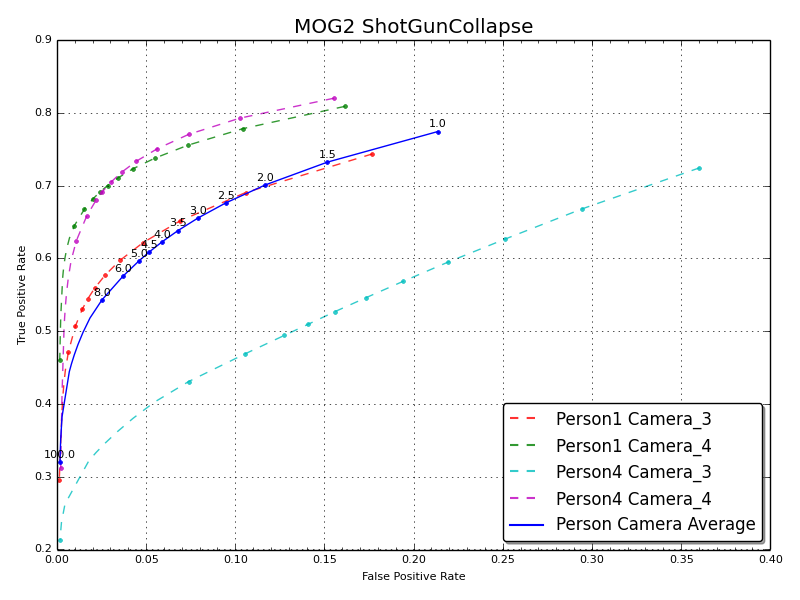
\includegraphics[width=80mm]{img/ap2/MOG2/SHOTGUNCOLLAPSE_P-C_1-1}}
\subfigure[WalkTurnBack]
{\label{fig:MOG2_WalkTurnBack}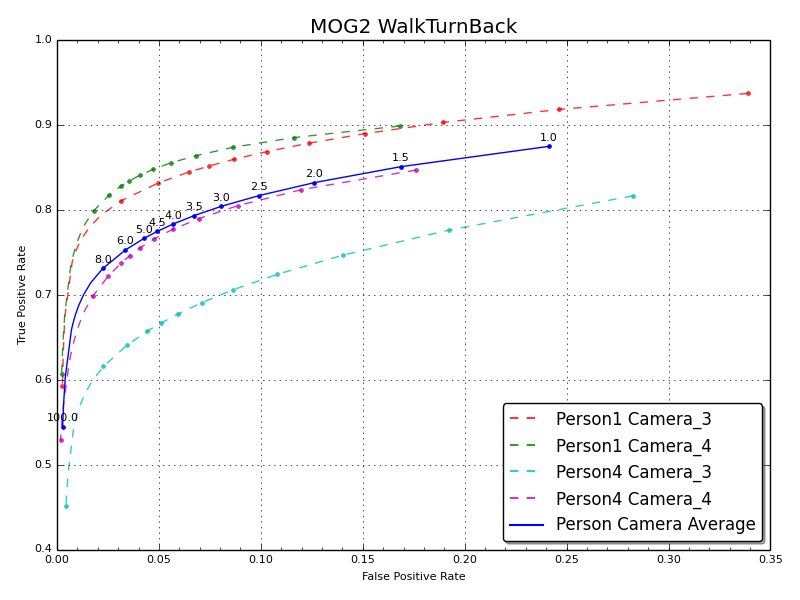
\includegraphics[width=80mm]{img/ap2/MOG2/WALKTURNBACK_P-C_1-1}}
\caption[Gráfica resultado global algoritmo MOG2 consolidado por acción]{Resultado global separado por acción de algoritmo MOG2}
\label{fig:MOG2_actions}
\end{figure}


\begin{figure}[!ht]
\centering     %%% not \center
\subfigure[Person1 Camera3]%
{\label{fig:MOG2_P1C3}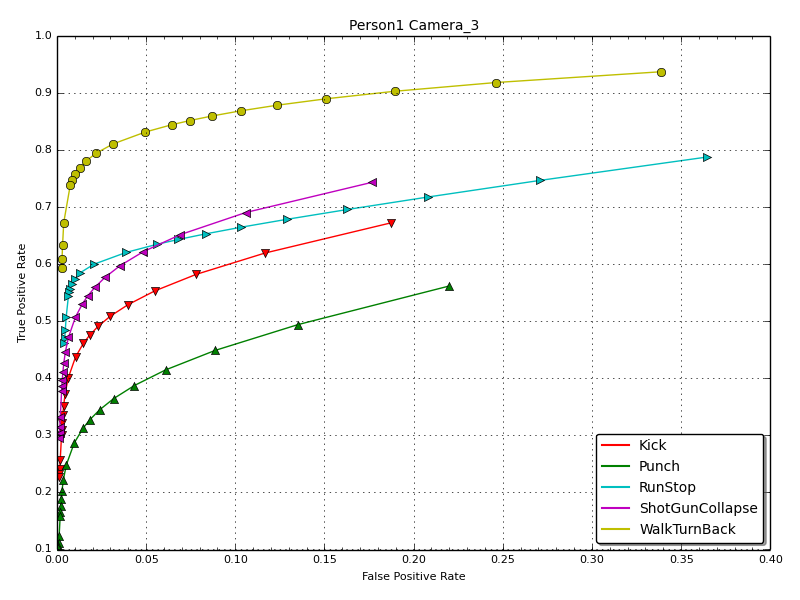
\includegraphics[width=80mm]{img/ap2/MOG2/P1C3}}
\subfigure[Person1 Camera4]
{\label{fig:MOG2_P1C4}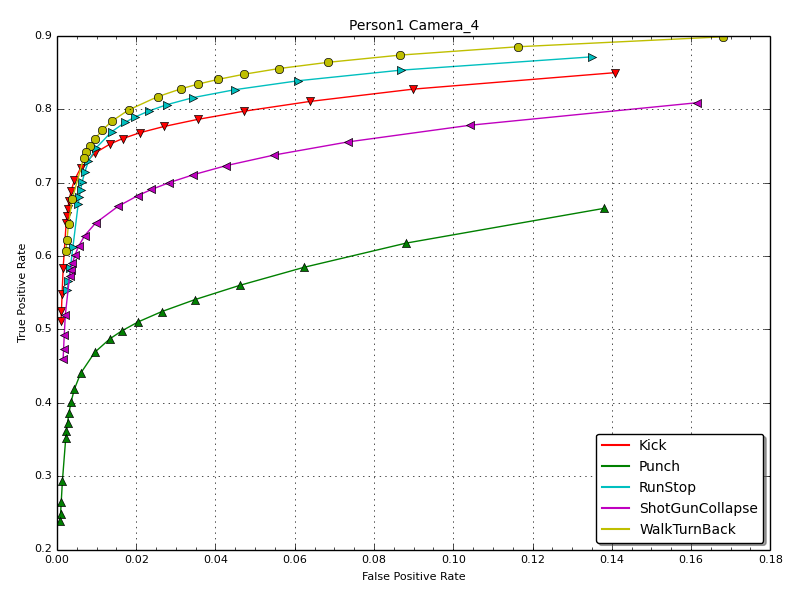
\includegraphics[width=80mm]{img/ap2/MOG2/P1C4}}
\subfigure[Person4 Camera3]
{\label{fig:MOG2_P4C3}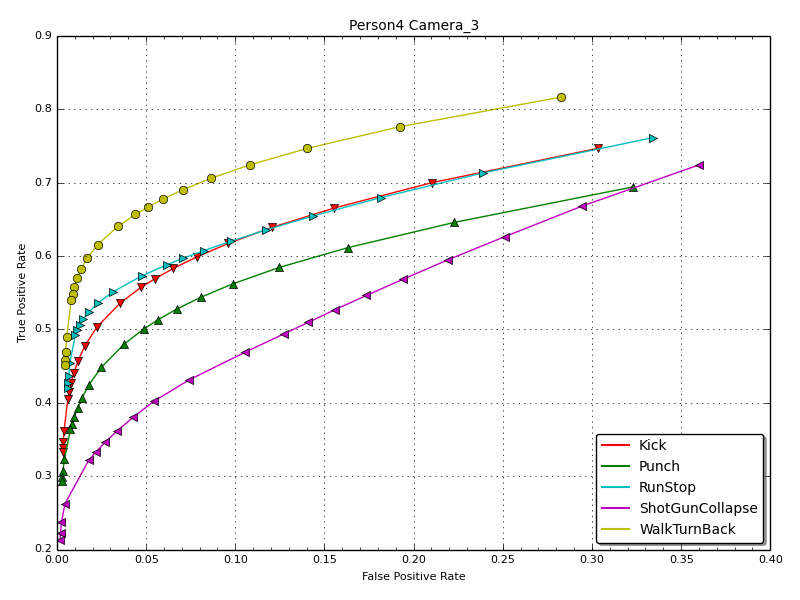
\includegraphics[width=80mm]{img/ap2/MOG2/P4C3}}
\subfigure[Person4 Camera4]
{\label{fig:MOG2_P4C4}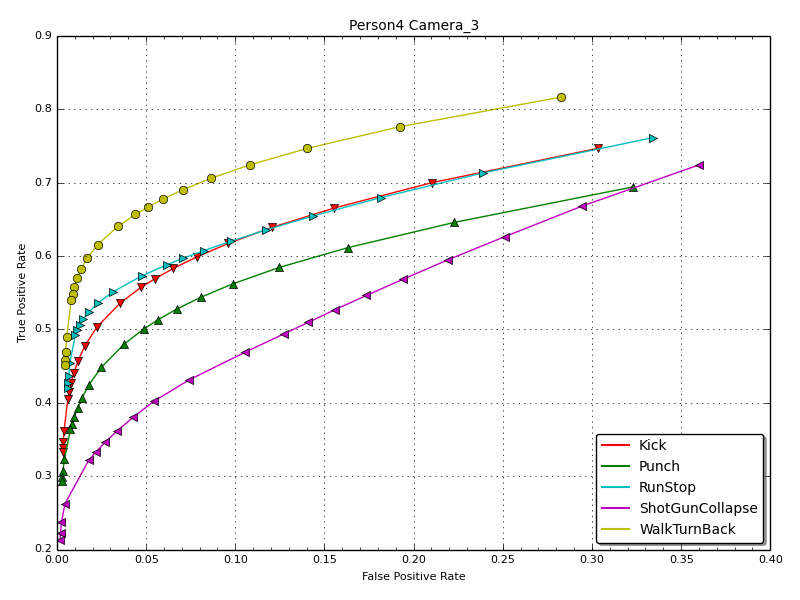
\includegraphics[width=80mm]{img/ap2/MOG2/P4C3}}
\caption[Resultados globales de la ejecución del algoritmo MOG2 separado por actor y camara.]{Resultados globales de la ejecución del algoritmo MOG2 separado por actor y camara. \textit{Person1} muestra un buen desempeño  }
\label{fig:MOG2_PC}
\end{figure}



%\begin{figure}[!ht]
%\centering     %%% not \center
%\subfigure[MCC ($\alpha=0.001$)]%
%{\label{fig:MCC-plot5-1_1}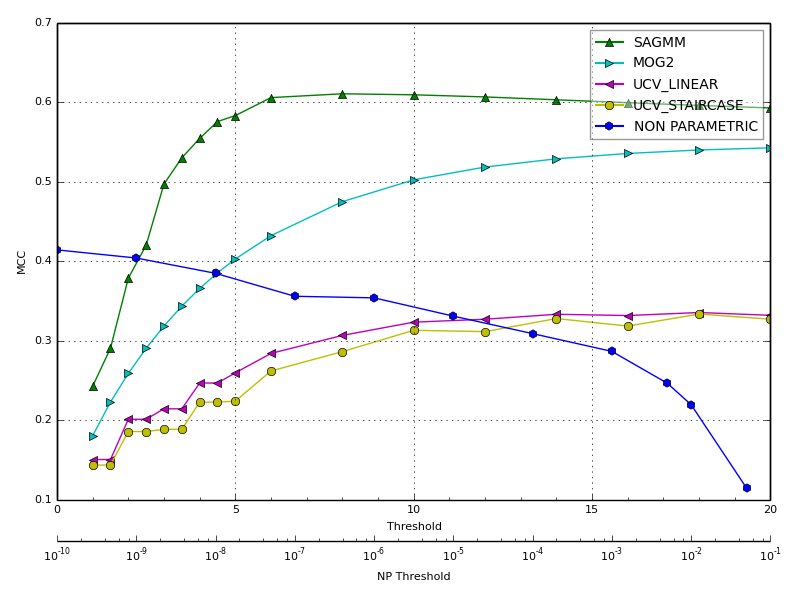
\includegraphics[width=80mm]{img/ap2/MCC-plot5-1_1}}
%\subfigure[MCC - Morfología ($\alpha=0.001$)]%
%{\label{fig:MCC-plot5-2_1}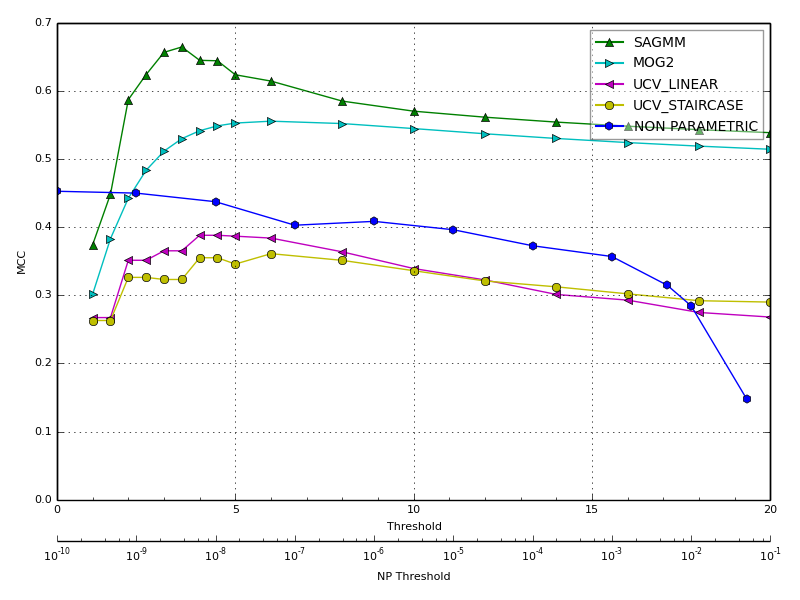
\includegraphics[width=80mm]{img/ap2/MCC-plot5-2_1}}
%\subfigure[FMeasure ($\alpha=0.001$)]%
%{\label{fig:FMeasure-plot5-1_1}\includegraphics[width=80mm]{img/ap2/FMeasure-plot5-1_1}}
%\subfigure[FMeasure - Morfología ($\alpha=0.001$)]%
%{\label{fig:FMeasure-plot5-2_1}\includegraphics[width=80mm]{img/ap2/FMeasure-plot5-2_1}}
%\subfigure[DScore ($\alpha=0.001$)]%
%{\label{fig:DSCORE-plot5-1_1}\includegraphics[width=80mm]{img/ap2/DSCORE-plot5-1_1}}
%\subfigure[DScore - Morfología ($\alpha=0.001$)]%
%{\label{fig:DSCORE-plot5-2_1}\includegraphics[width=80mm]{img/ap2/DSCORE-plot5-2_1}}
%\caption[Cuadros comparativos métricas de rendimiento de MCC, FMeasure, y DScore ($\alpha=0.001$).]{Cuadros comparativos generales de métricas de rendimiento MCC, FMeasure y DScore utilizando un factor de aprendizaje $\alpha=0.001$, con una instancia sin morfología y en una segunda instancia con morfología}
%\label{fig:ap2_metricas_1_1}
%\end{figure}
%
%
%\begin{figure}[!ht]
%\centering     %%% not \center
%\subfigure[PSNR ($\alpha=0.001$)]%
%{\label{fig:PSNR-plot5-1_1}\includegraphics[width=80mm]{img/ap2/PSNR-plot5-1_1}}
%\subfigure[PSNR - Morfología ($\alpha=0.001$)]%
%{\label{fig:PSNR-plot5-2_1}\includegraphics[width=80mm]{img/ap2/PSNR-plot5-2_1}}
%\subfigure[MSSIM ($\alpha=0.001$)]%
%{\label{fig:MSSIM-plot5-1_1}\includegraphics[width=80mm]{img/ap2/MSSIM-plot5-1_1}}
%\subfigure[MSSIM - Morfología ($\alpha=0.001$)]%
%{\label{fig:MSSIM-plot5-2_1}\includegraphics[width=80mm]{img/ap2/MSSIM-plot5-2_1}}
%\caption[Cuadros comparativos métricas de percepción PSNR y MSSIM ($\alpha=0.001$).]{Cuadros comparativos generales de métricas de percepción PSNR y MSSIM utilizando un factor de aprendizaje $\alpha=0.001$, en una primera experimentación sin morfología y en una segunda instancia con morfología}
%\label{fig:ap2_metricas_1_2}
%\end{figure}

%\begin{figure}[!ht]
%\centering     %%% not \center
%\subfigure[MCC ($\alpha=0.0002$)]%
%{\label{fig:MCC-plot5-2_1}\includegraphics[width=80mm]{img/ap2/MCC-plot5-2_1}}
%\subfigure[MCC - Morfología ($\alpha=0.001$)]%
%{\label{fig:MCC-plot5-2_2}\includegraphics[width=80mm]{img/ap2/MCC-plot5-2_2}}
%\subfigure[FMeasure ($\alpha=0.0002$)]%
%{\label{fig:FMeasure-plot5-2_1}\includegraphics[width=80mm]{img/ap2/FMeasure-plot5-2_1}}
%\subfigure[FMeasure - Morfología ($\alpha=0.0002$)]%
%{\label{fig:FMeasure-plot5-2_2}\includegraphics[width=80mm]{img/ap2/FMeasure-plot5-2_2}}
%\subfigure[DScore ($\alpha=0.0002$)]%
%{\label{fig:DSCORE-plot5-2_1}\includegraphics[width=80mm]{img/ap2/DSCORE-plot5-2_1}}
%\subfigure[DScore - Morfología ($\alpha=0.0002$)]%
%{\label{fig:DSCORE-plot5-2_2}\includegraphics[width=80mm]{img/ap2/DSCORE-plot5-2_2}}
%\caption[Cuadros comparativos métricas de rendimiento de MCC, FMeasure, y DScore ($\alpha=0.0002$).]{Cuadros comparativos generales de métricas de rendimiento MCC, FMeasure y DScore utilizando un factor de aprendizaje $\alpha=0.0002$, con una instancia sin morfología y en una segunda instancia con morfología}
%\label{fig:ap2_metricas_2_1}
%\end{figure}
%
%
%\begin{figure}[!ht]
%\centering     %%% not \center
%\subfigure[PSNR ($\alpha=0.0002$)]%
%{\label{fig:PSNR-plot5-2_1}\includegraphics[width=80mm]{img/ap2/PSNR-plot5-2_1}}
%\subfigure[PSNR - Morfología ($\alpha=0.001$)]%
%{\label{fig:PSNR-plot5-2_2}\includegraphics[width=80mm]{img/ap2/PSNR-plot5-2_2}}
%\subfigure[MSSIM ($\alpha=0.001$)]%
%{\label{fig:MSSIM-plot5-1_1}\includegraphics[width=80mm]{img/ap2/MSSIM-plot5-1_1}}
%\subfigure[MSSIM - Morfología ($\alpha=0.001$)]%
%{\label{fig:MSSIM-plot5-2_1}\includegraphics[width=80mm]{img/ap2/MSSIM-plot5-2_1}}
%\caption[Cuadros comparativos métricas de percepción PSNR y MSSIM ($\alpha=0.001$).]{Cuadros comparativos generales de métricas de percepción PSNR y MSSIM utilizando un factor de aprendizaje $\alpha=0.001$, en una primera experimentación sin morfología y en una segunda instancia con morfología}
%\label{fig:ap2_metricas_2_2}
%\end{figure}

